\documentclass[tikz,border=10pt]{standalone}
% Shared look for every TikZ diagram. Load with % Shared look for every TikZ diagram. Load with % Shared look for every TikZ diagram. Load with \input{../../tools/tikz-style.tex}
\usepackage[T1]{fontenc}
\usepackage{lmodern}
\renewcommand{\sfdefault}{lmr}  % diagrams use the same serif as the text
\usetikzlibrary{arrows.meta, positioning, shapes.geometric, calc, fit, backgrounds}
\definecolor{cblue}{HTML}{4C78A8}
\definecolor{corange}{HTML}{F58518}
\definecolor{cgreen}{HTML}{54A24B}
\definecolor{cred}{HTML}{E45756}
\definecolor{cpurple}{HTML}{B279A2}
\definecolor{cgrey}{HTML}{6B6B6B}
\tikzset{
  every picture/.style={font=\sffamily, line width=1.2pt},
  box/.style={draw=#1, fill=#1!12, rounded corners=4pt, align=center, inner sep=7pt, minimum height=1.1cm},
  box/.default=cgrey,
  arrow/.style={-{Stealth[length=3mm]}, draw=cgrey, line width=1.4pt},
  title/.style={font=\sffamily\bfseries\Large},
  note/.style={font=\sffamily\small, text=cgrey, align=center},
}
\AtBeginDocument{\hyphenpenalty=10000 \exhyphenpenalty=10000}

\usepackage[T1]{fontenc}
\usepackage{lmodern}
\renewcommand{\sfdefault}{lmr}  % diagrams use the same serif as the text
\usetikzlibrary{arrows.meta, positioning, shapes.geometric, calc, fit, backgrounds}
\definecolor{cblue}{HTML}{4C78A8}
\definecolor{corange}{HTML}{F58518}
\definecolor{cgreen}{HTML}{54A24B}
\definecolor{cred}{HTML}{E45756}
\definecolor{cpurple}{HTML}{B279A2}
\definecolor{cgrey}{HTML}{6B6B6B}
\tikzset{
  every picture/.style={font=\sffamily, line width=1.2pt},
  box/.style={draw=#1, fill=#1!12, rounded corners=4pt, align=center, inner sep=7pt, minimum height=1.1cm},
  box/.default=cgrey,
  arrow/.style={-{Stealth[length=3mm]}, draw=cgrey, line width=1.4pt},
  title/.style={font=\sffamily\bfseries\Large},
  note/.style={font=\sffamily\small, text=cgrey, align=center},
}
\AtBeginDocument{\hyphenpenalty=10000 \exhyphenpenalty=10000}

\usepackage[T1]{fontenc}
\usepackage{lmodern}
\renewcommand{\sfdefault}{lmr}  % diagrams use the same serif as the text
\usetikzlibrary{arrows.meta, positioning, shapes.geometric, calc, fit, backgrounds}
\definecolor{cblue}{HTML}{4C78A8}
\definecolor{corange}{HTML}{F58518}
\definecolor{cgreen}{HTML}{54A24B}
\definecolor{cred}{HTML}{E45756}
\definecolor{cpurple}{HTML}{B279A2}
\definecolor{cgrey}{HTML}{6B6B6B}
\tikzset{
  every picture/.style={font=\sffamily, line width=1.2pt},
  box/.style={draw=#1, fill=#1!12, rounded corners=4pt, align=center, inner sep=7pt, minimum height=1.1cm},
  box/.default=cgrey,
  arrow/.style={-{Stealth[length=3mm]}, draw=cgrey, line width=1.4pt},
  title/.style={font=\sffamily\bfseries\Large},
  note/.style={font=\sffamily\small, text=cgrey, align=center},
}
\AtBeginDocument{\hyphenpenalty=10000 \exhyphenpenalty=10000}

\begin{document}
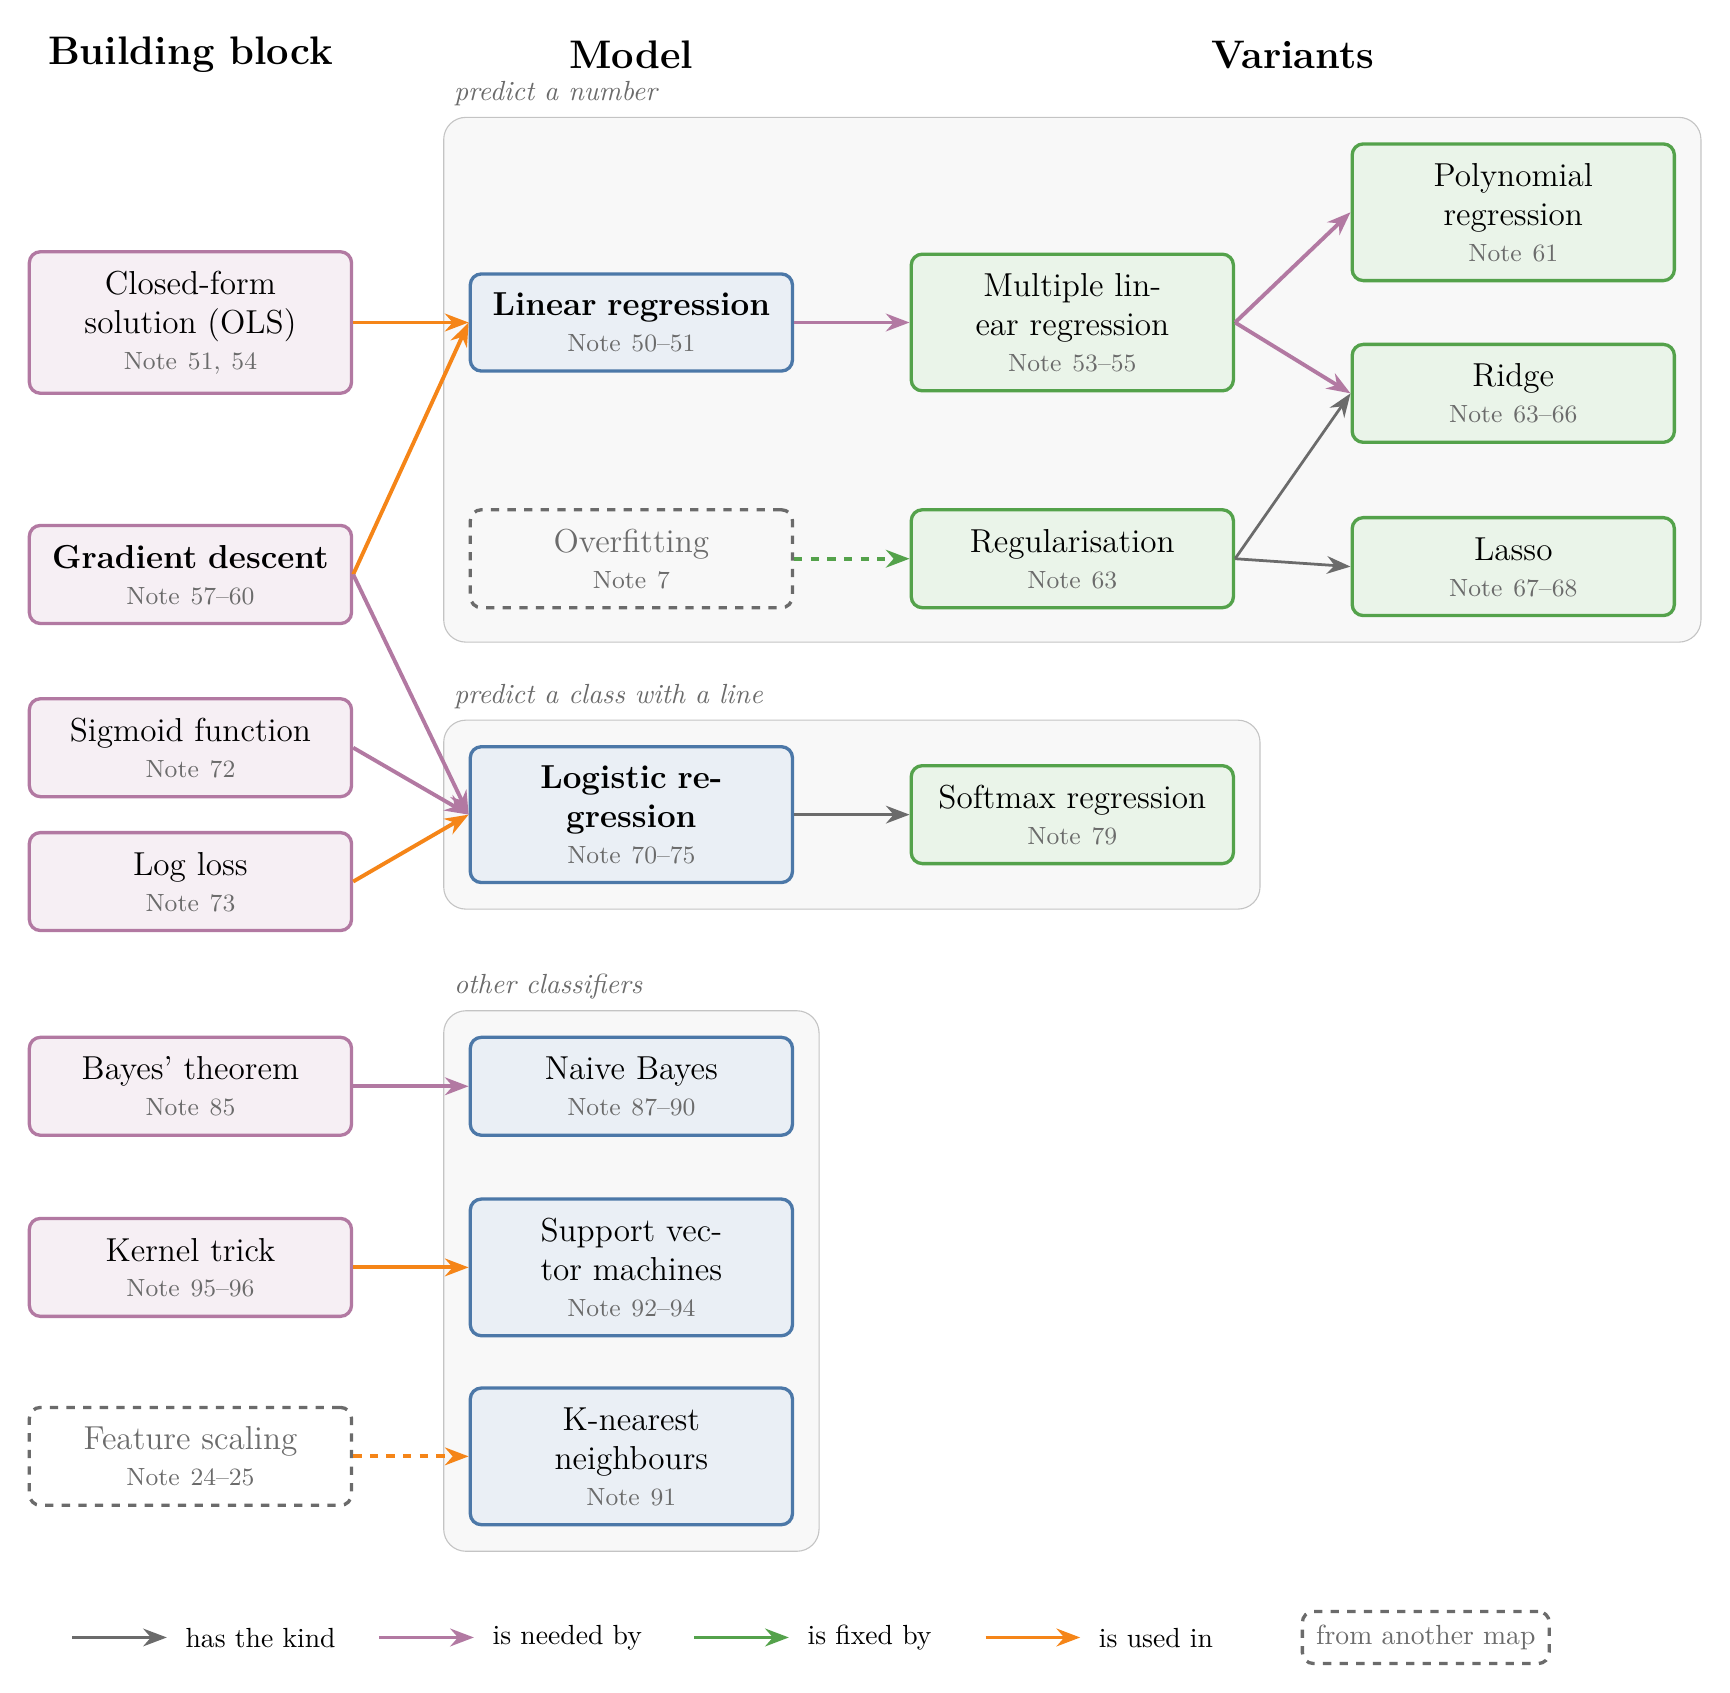
\begin{tikzpicture}[
    every node/.append style={font=\sffamily\large},
    blk/.style={box=cpurple, text width=3.6cm},
    mod/.style={box=cblue, text width=3.6cm},
    var/.style={box=cgreen, text width=3.6cm},
    prev/.style={draw=cgrey, dashed, rounded corners=4pt, align=center, inner sep=7pt, text=cgrey, text width=3.6cm, minimum height=1.1cm},
    group/.style={draw=cgrey!40, fill=cgrey!5, rounded corners=8pt, inner sep=9pt},
    gname/.style={font=\sffamily\normalsize\itshape, text=cgrey, anchor=south west},
    kindof/.style={arrow, draw=cgrey, line width=1pt},
    needs/.style={arrow, draw=cpurple},
    fixes/.style={arrow, draw=cgreen},
    usedin/.style={arrow, draw=corange},
  ]
  \newcommand{\nt}[1]{\\[-1pt]{\small\color{cgrey}Note #1}}
  \node[title] at (0,12.4)    {Building block};
  \node[title] at (5.6,12.4)  {Model};
  \node[title] at (14,12.4)   {Variants};

  % building blocks
  \node[blk] (ols)  at (0,9.0)  {Closed-form solution (OLS)\nt{51, 54}};
  \node[blk] (gd)   at (0,5.8)  {\textbf{Gradient descent}\nt{57--60}};
  \node[blk] (sig)  at (0,3.6)  {Sigmoid function\nt{72}};
  \node[blk] (ll)   at (0,1.9)  {Log loss\nt{73}};
  \node[blk] (bay)  at (0,-0.7) {Bayes' theorem\nt{85}};
  \node[blk] (ker)  at (0,-3.0) {Kernel trick\nt{95--96}};
  \node[prev] (sca) at (0,-5.4) {Feature scaling\nt{24--25}};

  % linear regression family
  \node[mod] (lin) at (5.6,9.0)  {\textbf{Linear regression}\nt{50--51}};
  \node[var] (mlr) at (11.2,9.0) {Multiple linear regression\nt{53--55}};
  \node[var] (pol) at (16.8,10.4) {Polynomial regression\nt{61}};
  \node[var] (rid) at (16.8,8.1) {Ridge\nt{63--66}};
  \node[var] (las) at (16.8,5.9) {Lasso\nt{67--68}};
  \node[var] (reg) at (11.2,6.0) {Regularisation\nt{63}};
  \node[prev] (ovr) at (5.6,6.0) {Overfitting\nt{7}};
  \draw[usedin] (ols) -- (lin);
  \draw[usedin] (gd.east) -- (lin.west);
  \draw[needs] (lin) -- (mlr);
  \draw[needs] (mlr.east) -- (pol.west);
  \draw[needs] (mlr.east) -- (rid.west);
  \draw[kindof] (reg.east) -- (rid.west);
  \draw[kindof] (reg.east) -- (las.west);
  \draw[fixes, dashed] (ovr) -- (reg);

  % logistic regression family
  \node[mod] (log) at (5.6,2.75) {\textbf{Logistic regression}\nt{70--75}};
  \node[var] (sof) at (11.2,2.75) {Softmax regression\nt{79}};
  \draw[needs] (gd.east) -- (log.west);
  \draw[needs] (sig.east) -- (log.west);
  \draw[usedin] (ll.east) -- (log.west);
  \draw[kindof] (log) -- (sof);

  % other classifiers
  \node[mod] (nb)  at (5.6,-0.7) {Naive Bayes\nt{87--90}};
  \node[mod] (svm) at (5.6,-3.0) {Support vector machines\nt{92--94}};
  \node[mod] (knn) at (5.6,-5.4) {K-nearest neighbours\nt{91}};
  \draw[needs] (bay) -- (nb);
  \draw[usedin] (ker) -- (svm);
  \draw[usedin, dashed] (sca) -- (knn);

  \begin{scope}[on background layer]
    \node[group, fit=(lin) (pol) (las) (ovr)] (g1) {};
    \node[group, fit=(log) (sof)] (g2) {};
    \node[group, fit=(nb) (knn)] (g3) {};
  \end{scope}
  \node[gname] at (g1.north west) {predict a number};
  \node[gname] at (g2.north west) {predict a class with a line};
  \node[gname] at (g3.north west) {other classifiers};

  % legend
  \begin{scope}[shift={(-1.5,-7.7)}, every node/.style={font=\sffamily, anchor=west}]
    \draw[kindof] (0,0) -- (1.2,0);   \node at (1.3,0) {has the kind};
    \draw[needs] (3.9,0) -- (5.1,0);  \node at (5.2,0) {is needed by};
    \draw[fixes] (7.9,0) -- (9.1,0);  \node at (9.2,0) {is fixed by};
    \draw[usedin] (11.6,0) -- (12.8,0); \node at (12.9,0) {is used in};
    \node[draw=cgrey, dashed, rounded corners=4pt, inner sep=5pt, text=cgrey, anchor=west] at (15.6,0) {from another map};
  \end{scope}
\end{tikzpicture}
\end{document}
